\documentclass[11pt,english]{article}

\usepackage[english]{babel}
\usepackage{enumitem}
\usepackage{fancyhdr}
\usepackage[top=2.3cm, bottom=2.3cm, left=1.6cm, right=1.6cm]{geometry}
\usepackage{graphicx}
\usepackage{lastpage}
\usepackage{tabularx}
\usepackage{listings}
\usepackage{color}
\usepackage{eurosym}

\definecolor{dkgreen}{rgb}{0,0.6,0}
\definecolor{gray}{rgb}{0.5,0.5,0.5}
\definecolor{mauve}{rgb}{0.58,0,0.82}

\lstset{frame=tb,
	language=SQL,
	aboveskip=3mm,
	belowskip=3mm,
	showstringspaces=false,
	columns=flexible,
	basicstyle={\small\ttfamily},
	numbers=none,
	numberstyle=\tiny\color{gray},
	keywordstyle=\color{blue},
	commentstyle=\color{dkgreen},
	stringstyle=\color{mauve},
	breaklines=true,
	breakatwhitespace=true,
	tabsize=3
}

\pagestyle{fancy}
\setlength{\parindent}{0pt}        % indentation on new paragraph
\setlength{\parskip}{0pt}          % vertical spacing on new paragraph
\setlength{\lineskip}{1pt}         % vertical spacing between lines
\setlength{\columnsep}{1cm}        % spacing between columns
\setlength{\belowcaptionskip}{0pt} % spacing below captions
\setlength{\abovecaptionskip}{5pt} % spacong above captions

\graphicspath{{assets/}}

\lfoot{}
\cfoot{\today}
\rfoot{\thepage/\pageref{LastPage}}

\newcommand*{\Frontpage}{\begingroup
	\hbox{%
		\hspace*{0.2\textwidth}
		\rule{1pt}{\textheight}
		\hspace*{0.05\textwidth}
		\parbox[b]{0.75\textwidth}{%
			{\noindent\Huge\bfseries DATAB3}\\[2\baselineskip] % Title
			{\large \textit{Huiswerkopdrachten, week 4}}\\[4\baselineskip] % Tagline or further description
			{\Large \textsc{\\
				Patrick Spek, 2099745 \\
				Chris Meesters, 2098474 \\
			}}
			\vspace{0.5\textheight} % Whitespace between the title block and the publisher
		}
	}
\endgroup}

\renewcommand{\footrulewidth}{0.4pt}

\begin{document}
	\thispagestyle{empty}
	\Frontpage

	\newpage
	\tableofcontents

	\newpage
	\section{bereken\_rente}
	\begin{lstlisting}
CREATE OR REPLACE TRIGGER "LENING_BRI"

BEFORE
INSERT ON "LENING"
FOR EACH ROW
DECLARE
	NieuweSleutel_ integer;
	Resultaat VARCHAR2(255);
	Fout EXCEPTION;

BEGIN
	SELECT nvl(max(ln.number), 0)
	INTO NieuweSleutel_
	FROM lening ln;
	--

	Resultaat := CHECK_NAAM_LENING(:new.GELEENDVAN, :new.GELEENDAAN);
	IF Resultaat <> 'NORMAAL' THEN
		RAISE Fout;
	END IF;

	NieuweSleutel_ = NieuweSleutel_ + 1;
	:new.nummer = NieuweSleutel_;

	EXCEPTION
	WHEN Fout THEN
		apex_error.add_error (
			p_message => Resultaat,
			p_additional_info => null,
			p_display_location => apex_error.c_error_on_page
		);
END
	\end{lstlisting}

	\newpage
	\section{Schermafdrukken}
	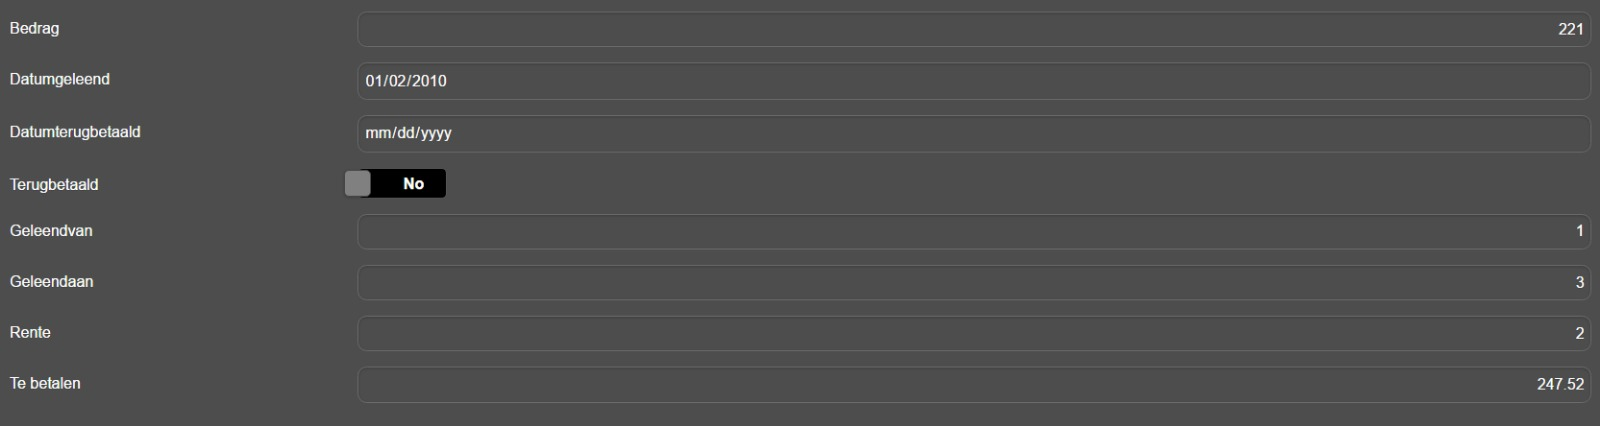
\includegraphics[scale=0.5]{week4-img1}

	\newpage
	\section{Controle functio}
	\begin{lstlisting}
CREATE OR REPLACE FUNCTION "BEREKEN_RENTE"
(
	in_bedrag IN NUMBER,
	in_rente IN NUMBER,
	in_datumgeleend IN DATE
) RETURN NUMBER
IS
	jaar INTEGER;
	bedrag INTEGER;
BEGIN
	jaar := floor(months_between(sysdate, in_datumgeleend) / 12);
	bedrag := in_bedrag + in_bedrag * (in_rente / 100) * jaar;

	RETURN bedrag;
END
	\end{lstlisting}

	\newpage
	\section{Trigger}
	\begin{lstlisting}
CREATE OR REPLACE FUNCTION "CHECK_NAAM_LENING"
(
	in_uitlener NUMBER,
	in_lener NUMBER
) RETURN VARCHAR2
IS resultaat VARCHAR2(255);

BEGIN
	IF in_uitlener = in_lener THEN
		resultaat := "De lener en de uitlener kunnen niet dezelfde persoon zijn.";
	ELSE
		resultaat := "Normaal";
	END IF;

	RETURN resultaat;
END;
	\end{lstlisting}

	\newpage
	\section{Schermafdrukken}
	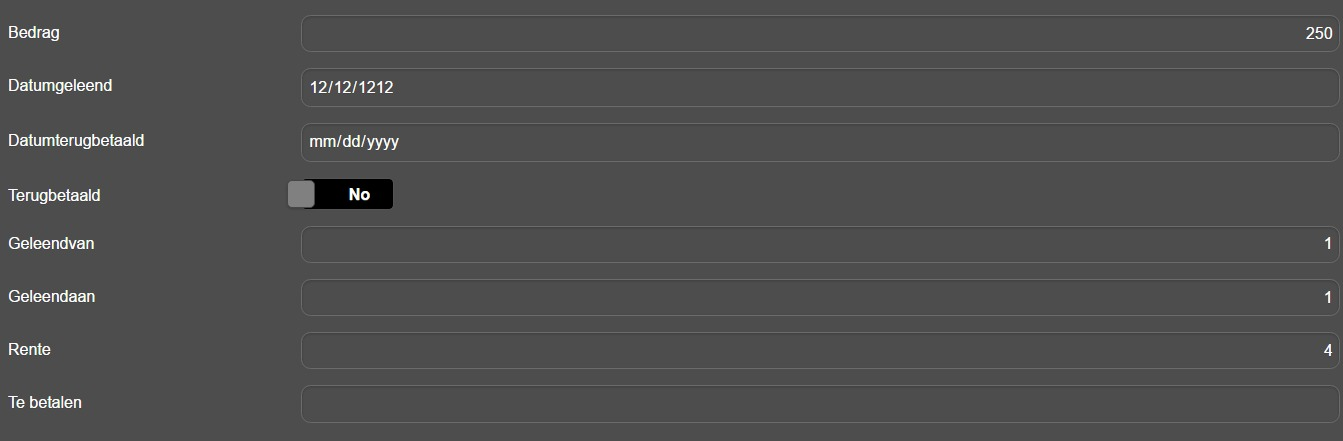
\includegraphics[scale=0.5]{week4-img2}

	\newpage
	
\includegraphics[scale=0.5]{week4-img3}

	\newpage
	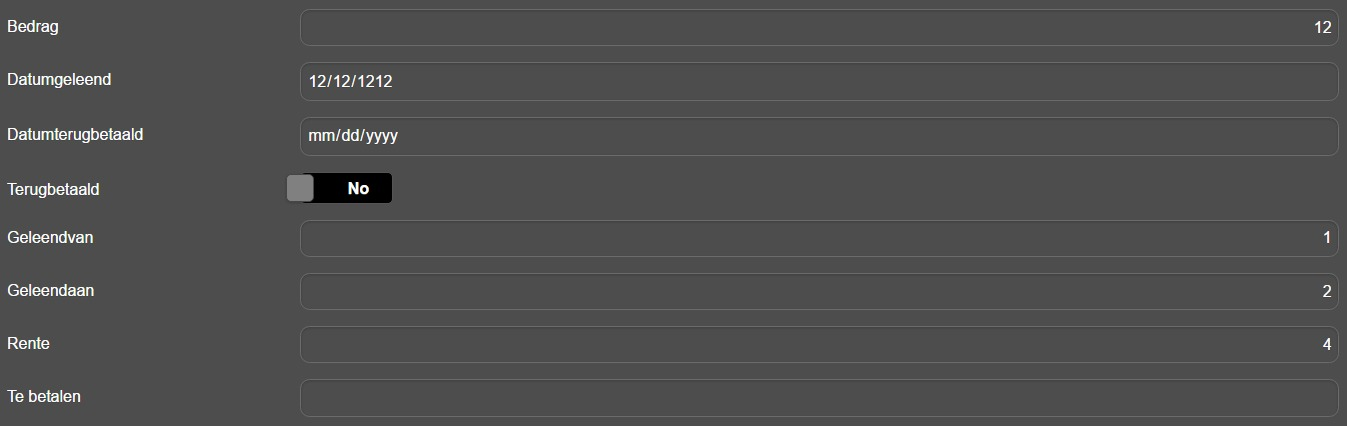
\includegraphics[scale=0.5]{week4-img4}

	\newpage
	
\includegraphics[scale=0.5]{week4-img5}
\end{document}

